\documentclass[sigconf,authorversion,nonacm]{acmart}

\usepackage{tikz}
\usepackage{subcaption}

\begin{document}
\title{Project Design Paper}
\subtitle{Team 4: LDA}

\author{Webi Tesfaye Dabuse}
\authornote{Team Leader}
\affiliation{
    \institution{KAIST}
    \city{Daejeon}
    \country{South Korea}
}
\email{webby@kaist.ac.kr}

\author{Melka Dawit Legesse}
\affiliation{
    \institution{KAIST}
    \city{Daejeon}
    \country{South Korea}
}
\email{kaidavid7@kaist.ac.kr}

\author{Ohjun Kwon}
\affiliation{
    \institution{KAIST}
    \city{Daejeon}
    \country{South Korea}
}
\email{ohjun@kaist.ac.kr}

\begin{abstract}
    Our project focuses on implementing the text mining concepts and techniques we have learnt in our CS474 - Text Mining class. The provided dataset contains news articles from Korea news article outlets that were reported over a three years period - 2015, 2016, and 2017.

    In this project proposal, we briefly discuss the approaches (Clustering, IR, …) and tools (SpaCy, BERT, GloVe, ... ) we are planning to use to analyze and track trending issues of the given dataset.  In the meantime, our current approaches are subject to change at any time.
\end{abstract}

\maketitle

\section{Introduction}
Text data holds the most part of unstructured data that, by itself,  accounts for 80\% of all the existing data, and therefore it is a rich source for data analytics and AI application deployments making Text Mining an essential field. Furthermore, Text Mining draws upon several related fields such as IR, Data Mining, NLP, and others. Its aim of automatically identifying patterns within raw text are achieved through text/ document categorization, summarization, clustering, sentiment analysis, entity relation modeling and so on.

The first step of any Text Mining process is data gathering followed by understanding and preprocessing the gathered data before jumping to its analysis.

Here\footnote{\url{https://colab.research.google.com/drive/1USc3MSpSbJEzZ2H-y3pgnhGDS7JXUtR-}} is the source code for preliminary preprocessing and data visualizations.


\section{Problem Definition}
As news agencies continuously report what happens across the globe, they are great sources of text data. Their articles can be used to extract the most trending issues for a given time interval and to track some events through Text Mining. In this term project, we will be relying on Korean newspaper articles to accomplish these tasks.

\subsection{Issue Trend Analysis}
This task is to rank the top ten most significant issues
that have been observed in the given news dataset
which includes news articles of three years(2015-2017).
However, there are many ambiguities in the task.
In order to express accurately as an algorithm,
the task must be clearly defined.

\paragraph{Significance measure}
First, let's define what is meant by \emph{a significant issue},
which is the most central concept of this task.
We should be very specific about what a significant issue means
and a measure of the significance of a given issue should be defined well.
A definite quantitative measure is needed
in order to compare significancies among issues.
We can determine the significance of an issue
with the number of related news articles,
or the duration that certain issue has been covered by news articles.
However, if a specific issue is covered for a long period of time,
the number of related news articles will generally increase,
so the number of related news articles includes some factors of the duration.
Furthermore, if a follow-up article on a particular issue is written after a long period of time,
this data can make a bias in the result.

\begin{figure}[h]
    \centering
    \vspace*{5mm}
    \begin{subfigure}{0.5\linewidth}
        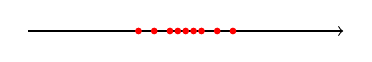
\begin{tikzpicture}
            \draw [->] (0,0) -- (4,0);
            \filldraw [red] (1.4,0) circle (1pt);
            \filldraw [red] (1.6,0) circle (1pt);
            \filldraw [red] (1.8,0) circle (1pt);
            \filldraw [red] (1.9,0) circle (1pt);
            \filldraw [red] (2,0) circle (1pt);
            \filldraw [red] (2.1,0) circle (1pt);
            \filldraw [red] (2.2,0) circle (1pt);
            \filldraw [red] (2.4,0) circle (1pt);
            \filldraw [red] (2.6,0) circle (1pt);
        \end{tikzpicture}
        \vspace*{5mm}
        \subcaption{Dense}
        \label{fig:dense}
    \end{subfigure}%
    \begin{subfigure}{0.5\linewidth}
        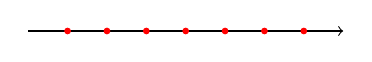
\begin{tikzpicture}
            \draw [->] (0,0) -- (4,0);
            \filldraw [red] (0.5,0) circle (1pt);
            \filldraw [red] (1,0) circle (1pt);
            \filldraw [red] (1.5,0) circle (1pt);
            \filldraw [red] (2,0) circle (1pt);
            \filldraw [red] (2.5,0) circle (1pt);
            \filldraw [red] (3,0) circle (1pt);
            \filldraw [red] (3.5,0) circle (1pt);
        \end{tikzpicture}
        \vspace*{5mm}
        \subcaption{Sparse}
        \label{fig:sparse}
    \end{subfigure}
    \caption{Two different examples of published articles lined up in a chronological order}
\end{figure}

Even in a short period of time, if a lot of related articles were published,
the issue would have been of high significance.
It can be inferred that issues that people have encountered relatively frequently
even in a short period of time(Figure~\ref{fig:dense})
will be more memorable to people
than issues encountered intermittently
over a long period of time(Figure~\ref{fig:sparse}).
Therefore, let's define a significant issue as an issue
which has lots of related articles.

\paragraph{Clustering}
We can determine what is a significant issue by the number of related articles.
Then, how to group \emph{related articles} becomes a very important issue.
We will perform topic analysis, which extracts main topic information from
the collections of articles, and perform trend analysis which observes
extracted topics chronologically.
We will talk about topic analysis in the topic modeling paragraph, and
let's focus on the trend analysis.
We need to decide whether we want to extract topics first on the whole three years of articles,
or extract topics from each year. The former method is useful when we want to
focus on the changes and transitions of the topics, and the latter method is
useful when we want to differentiate each year and compare among them.
In our task, the latter method will suit perfectly.

\paragraph{Preprocessing}
Before we start to process articles with the models, we need to preprocess the
article texts.
For instance, we need to filter irrelevant texts like tags, symbols, math symbols, or punctuations.
Also, we need to remove stopwords, and stemming of the words should be done.

\paragraph{Topic Modeling}
As we saw while defining the task above,
since this work can be viewed as a type of topic modeling problem,
the problem can be solved using related models.
For the methods for topic modeling,
a basic model called LSA(Latent Semantic Analysis)
was introduced by Deerwester(1990)\cite{deerwester1990indexing}.
After that, Hofmann(1999) proposed PLSA(Probabilistic Latent Semantic Analysis) which
introduced probabilistic concept to LSA\cite{hofmann1999probabilistic}.
Recently, LDA(Latent Dirichlet Allocation) proposed by Blei et al.(2003)\cite{blei2003latent}
has been used in various fields,
furthermore, BERT proposed by Devlin(2019)\cite{devlin2019bert} has become a building foundation
of state-of-the-art models.

\subsection{Issue Tracking}
\subsubsection{On-issue Event Tracking}
\label{sec:onissue}
This task involves listing the events related to the issue in question on a temporal line. News articles contain many events that are most likely mentioned in another article. Articles usually embed links to other articles that are related to them using their titles on the body section making it easier to hop from one article to the other while going back on the temporal line.

\begin{figure}[h]
    \centering
    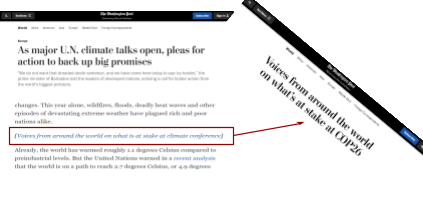
\includegraphics[width=\linewidth]{img/rel.png}
    \caption{Relation between events in news articles}
\end{figure}

However, going through the Yonhap News Agency page, this is not true and they have their own \emph{`Related Articles'} and \emph{`Keywords'} section at the bottom of their pages which are not included in the given dataset. Were it given, the task of finding relation between articles would be simplified.

As an alternative approach we can start by clustering all the articles using k-means clustering or LDA topic modeling so that the articles with the most similarity will group together to create a smaller pool of documents. This phase will collect related articles together and it will be easier to check the similarity between events in these documents. After the clusters are made, we will query the issues to get the most suitable cluster for a specific issue. This might be a bad assumption as the clustering is unsupervised; however, we will experiment on this approach using different parameters (e.g. k in k-means clustering). Although there is no guarantee in the direct correlation of the events in these clusters, we will have a better chance of finding many on-issue events.

We are planning to use Transformer-based event-extraction tools (we haven’t decided which one yet) to get the events inside documents in the clusters. This task is difficult and computationally expensive. After getting the events inside each document related to the issue in question, we will use relation extraction methods to see the detailed information of these events. The relation extraction task can be done using BERT-based models or Spacy.

\begin{figure}[h]
    \centering
    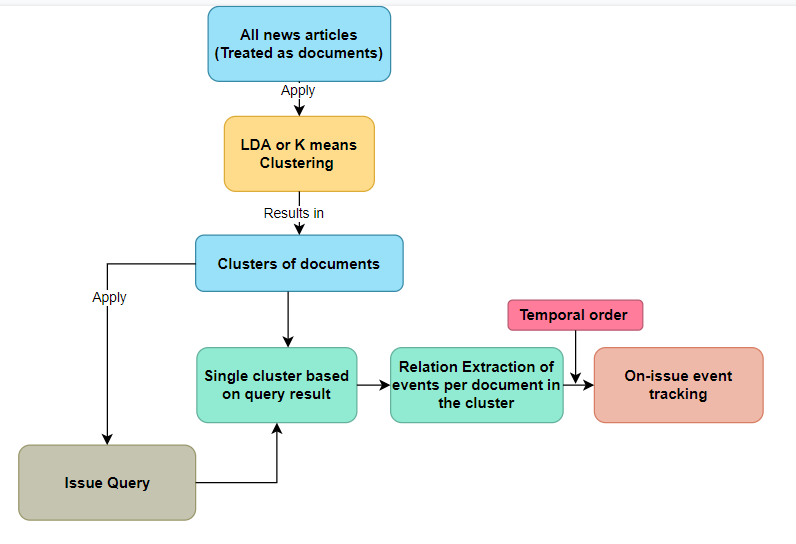
\includegraphics[width=\linewidth]{img/2-1pipeline.png}
    \caption{Pipeline for task \ref{sec:onissue}}
\end{figure}


\subsubsection{Related-issue Event Tracking}
After finding the top issues of each year and automatically extracting detailed information from two issues which are the most suitable for such analyses, we will be identifying other events that are related to them but not directly tied.

Assuming that we have these two issues and the documents that best represent them, we will first extract intra-document (inter-sentence) relations in terms of \emph{time, places}, and \emph{participants}. Any other document we extract shouldn’t have inter-sentence relations that are linked to these factors.
\begin{figure}[h]
    \centering
    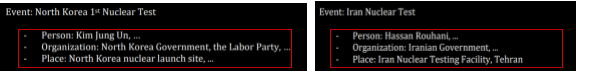
\includegraphics[width=\linewidth]{img/2-2.png}
\end{figure}

None of the above red bounded outputs should be the same for Related-Issue Event Tracking. Moreover, at this stage, we shouldn’t rely on the timeframe of the issue.

However, we can rely on the \emph{document similarity} between the document that best represents the issues and any other documents (starting with documents within the same cluster) while checking the difference in their inter-sentence relations.
i.e. Maximize document similarity while minimizing similarity between the inter-sentence relations of the documents


\paragraph{Document Similarity}
The distance between two documents can be used as a key factor for information retrieval and the different methods that are implemented are: Jaccard distance, Cosine distance, Euclidean distance, and Relaxed Word Mover’s distance with Cosine and Euclidean being the most common and effective for documents represented in vector space. Additionally, the different embedding techniques that are used to represent a document as a vector are: Tf-Idf, Word2Vec, GloVe, Doc2Vec, and BERT.

\section{Related Works}
\paragraph{Structure Self-Attention Network (SSAN)}
a novel extension of Transformer to effectively incorporate structural dependencies between input elements.

\paragraph{RoBERTa-Large}
A Robustly Optimized BERT Pretraining Approach with 24-layer, 1024-hidden, 16-heads, 355M parameters RoBERTa using the BERT-large architecture.

\paragraph{SSAN-RoBERTa-Large + Adaptation}
This model is used for inter-sentence or document level relations as it showed the highest performance on DocRED dataset.

\paragraph{DocRED}
DocRED is a large-scale document-level relation extraction dataset constructed from Wikipedia and Wikidata with three features:
\begin{itemize}
    \item Annotates both named entities and relations, and is the largest human-annotated dataset for document-level RE from plain text
    \item Requires reading multiple sentences in a document to extract entities and infer their relations by synthesizing all information of the document
    \item Can be adopted for both supervised and weakly supervised scenarios.
\end{itemize}

\begin{figure}[h]
    \centering
    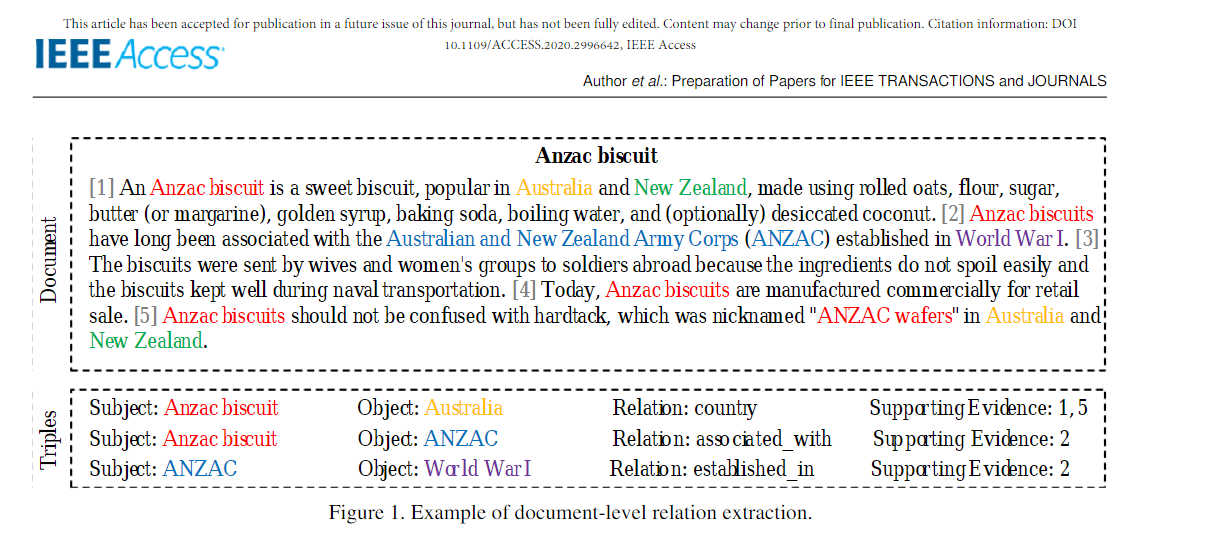
\includegraphics[width=\linewidth]{img/relax.png}
    \caption{Example of document-level relation extraction on a paragraph}
\end{figure}

\section{Intermediate Results}
In an attempt to understand the content of the news articles in the documents, we performed preliminary data cleaning and visualization. As the given dataset is divided into 8 files, we started by concatenating them. To categorize the news articles, we used the ‘section’ column. Figure~\ref{fig:graph} shows the number of articles from each section in the span of three years. As observed from the graph, ‘Social Affairs’ - 7,233 articles, ‘North Korea’ - 5,497 articles, and ‘Politics’ - 4,409 articles are the three largest sections containing roughly 2,000 articles each per year. Sections such as ‘Sharing’ and ‘Environment’ are among the smallest sections.

\begin{figure}[h]
    \centering
    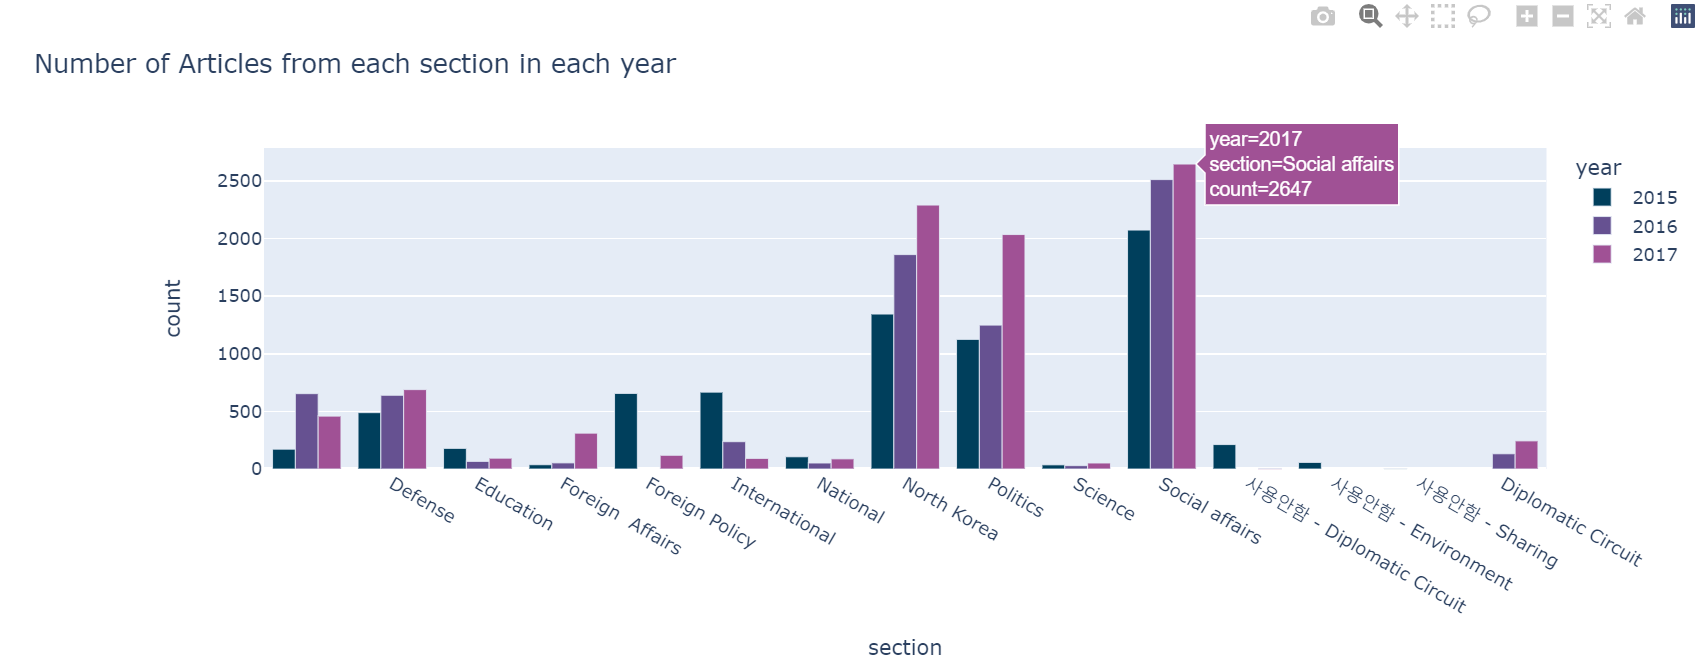
\includegraphics[width=\linewidth]{img/year.png}
    \caption{Graph showing the number of articles from each section in each year.}
    \label{fig:graph}
\end{figure}

To visualize the word-frequency based summary of the dataset, we used word clouds on the body and title of the news articles. Figure~\ref{fig:cloud} shows the word cloud pipeline.

\begin{figure}[h]
    \centering
    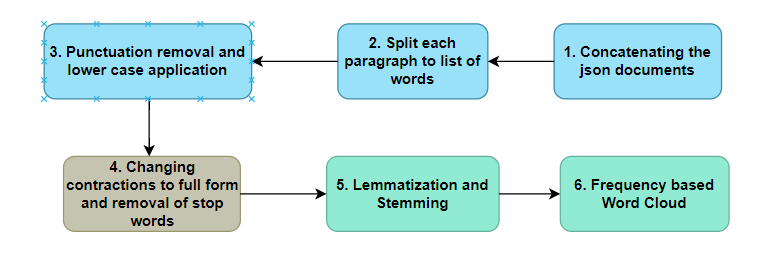
\includegraphics[width=\linewidth]{img/cloudpipeline.png}
    \caption{Pipeline for the word Cloud (Preprocessing)}
    \label{fig:cloud}
\end{figure}

\begin{figure}[h!]
    \begin{subfigure}{0.5\linewidth}
        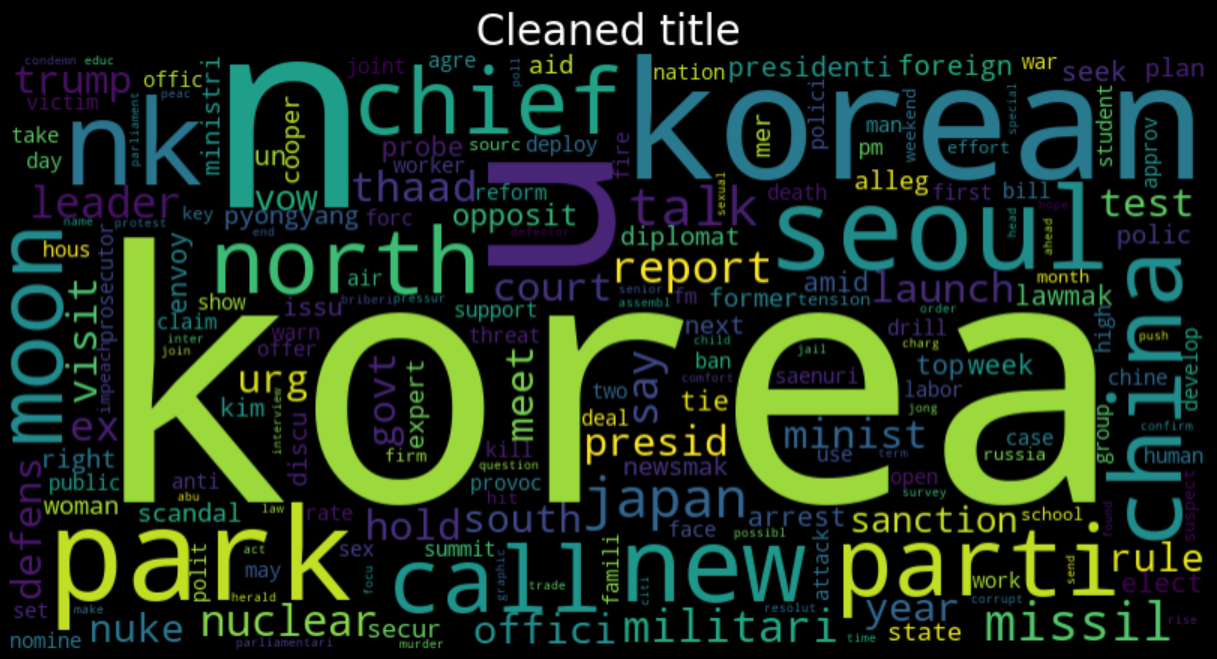
\includegraphics[width=0.9\linewidth]{img/title.png}
        \subcaption{Cleaned title}
    \end{subfigure}%
    \begin{subfigure}{0.5\linewidth}
        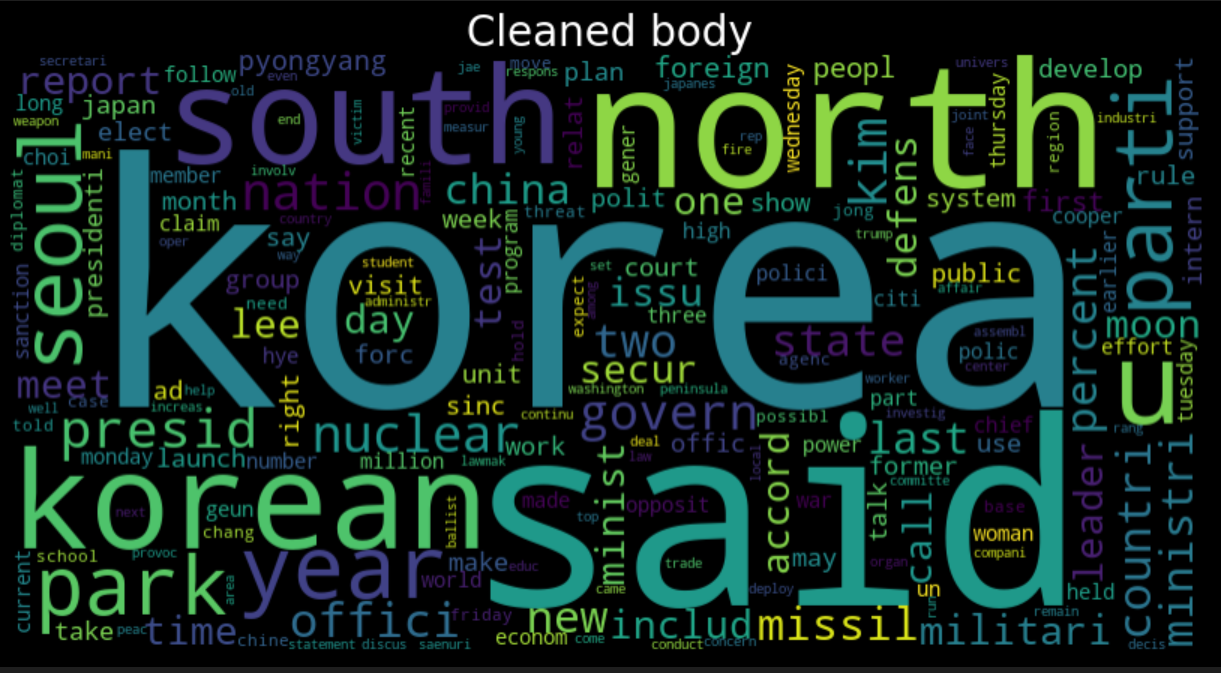
\includegraphics[width=0.9\linewidth]{img/body.png}
        \subcaption{Cleaned body}
    \end{subfigure}
    \caption{Word cloud based on body and title of every news article in the Korea Herald Dataset}
\end{figure}

\nocite{*}
\bibliographystyle{ACM-Reference-Format}
\bibliography{ref}

\end{document}